\section{Related work}
\begin{frame}[t]{Related work}
    \framesubtitle{Unsupervised methods}

    Mostly ranking techniques that use:
    \begin{itemize}
      \item<2->{language models}
      \item<3->{clusters}
      \item<4->{or \textbf{graphs} of word
                co-occurrences}
      \begin{itemize}
        \item<5->{weighted with co-occurrence number or semantic measure}
        \item<6->{refined with similar documents}
        \item<7->{biased with topic probabilities}
        \item<8->{modified to rank topics instead of words}
      \end{itemize}
    \end{itemize}
    \alt<8>{
      \begin{figure}
        \centering
        \newcount\mycount
        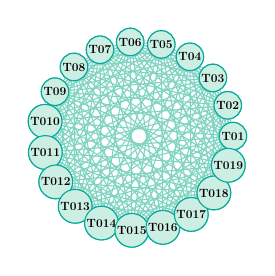
\begin{tikzpicture}[scale=.3,
                            align=center,
                            every node/.style={transform shape},
                            main node/.style={text centered,
                                              circle,
                                              draw=JungleGreen,
                                              fill=JungleGreen!20,
                                              inner sep=1.5pt,
                                              font=\Large\bfseries}]
          \foreach \number/\pos in {1/above,2/above,3/above,4/above,5/above,6/above,7/above,8/above,9/above,10/above,11/below,12/below,13/below,14/below,15/below,16/below,17/below,18/below,19/below}{
            \mycount=\number
            \advance\mycount by -1
            \multiply\mycount by 19
            \advance\mycount by 0
            \ifthenelse{\number > 9}{
              \node[main node] (N-\number) at (\the\mycount:4cm) {T\number};
            }{
              \node[main node] (N-\number) at (\the\mycount:4cm) {T0\number};
            }
          }
          \foreach \number in {1,...,18}{
            \mycount=\number
            \advance\mycount by 1
            \foreach \numbera in {\the\mycount,...,19}{
              \path[JungleGreen!50] (N-\number) edge (N-\numbera);
            }
          }
          \foreach \number/\pos in {1/above,2/above,3/above,4/above,5/above,6/above,7/above,8/above,9/above,10/above,11/below,12/below,13/below,14/below,15/below,16/below,17/below,18/below,19/below}{
            \mycount=\number
            \advance\mycount by -1
            \multiply\mycount by 19
            \advance\mycount by 0
            \ifthenelse{\number > 9}{
              \node[main node] (N-\number) at (\the\mycount:4cm) {T\number};
            }{
              \node[main node] (N-\number) at (\the\mycount:4cm) {T0\number};
            }
          }
        \end{tikzpicture}\\
        \cite[\underline{TopicRank}]{bougouin2013topicrank}
      \end{figure}
    }{
      \alt<7>{
        \vfill
        \begin{figure}
          \centering
          \begin{columns}
            \begin{column}{.24\linewidth}
              \centering
              \begin{tikzpicture}[thin,
                                  auto,
                                  scale=.175,
                                  align=center,
                                  node distance=1.25cm,
                                  every node/.style={font=\small, transform shape},
                                  main node/.style={text centered,
                                                    thick,
                                                    fill=JungleGreen!20,
                                                    inner sep=1.5pt,
                                                    font=\Large\bfseries}]
                % connected component
                \node[main node, fill=BurntOrange!50] (university) {university};
                \node[main node] (duke) [above left=of university.north] {duke};
                \node[main node] (library) [above=of university.north east] {library};
                \node[main node] (press) [below left=of university.south] {press};
                \node[main node] (cornell) [below right=of university.south] {cornell};

                \path[JungleGreen!50] (university) edge (library);
                \path[JungleGreen!50] (university) edge (duke);
                \path[JungleGreen!50] (university) edge (press);
                \path[JungleGreen!50] (university) edge (cornell);

                % connected component
                \node[main node] (further) [left=of university.south west] {further};
                \node[main node] (skills) [below=of further.south west] {skills};

                \path[JungleGreen!50] (skills) edge (further);

                % connected component
                \node[main node, fill=BurntOrange!50] (scholarly) [right=of library.north east] {scholarly};
                \node[main node] (communication) [below=of scholarly.west] {communication};
                \node[main node, fill=BurntOrange!50] (publishing) [below right=of scholarly.south] {publishing};
                \node[main node] (scene) [above right=of publishing.west] {scene};
                \node[main node] (initiative) [below=of publishing.west] {initiative};
                \node[main node, fill=BurntOrange!50] (journal) [below right=of scene.north east] {journal};
                \node[main node, fill=BurntOrange!50] (electronic) [below=of journal.east] {electronic};
                \node[main node] (joint) [below=of electronic.north west] {joint};

                \path[JungleGreen!50] (communication) edge (scholarly);
                \path[JungleGreen!50] (publishing) edge (scholarly);
                \path[JungleGreen!50] (publishing) edge (scene);
                \path[JungleGreen!50] (publishing) edge (journal);
                \path[JungleGreen!50] (publishing) edge (initiative);
                \path[JungleGreen!50] (journal) edge (electronic);
                \path[JungleGreen!50] (joint) edge (electronic);

                % connected component
                \node[main node] (new) [below=of skills.south] {new};
                \node[main node, fill=BurntOrange!50] (role) [below=of new.south east] {role};

                \path[JungleGreen!50] (new) edge (role);

                % connected component
                \node[main node] (digital) [right=of new.south east] {digital};
                \node[main node, fill=BurntOrange!50] (libraries) [below =of cornell.south] {libraries};
                \node[main node] (research) [right =of libraries.south east] {research};

                \path[JungleGreen!50] (digital) edge (libraries);
                \path[JungleGreen!50] (libraries) edge (research);

                % connected component
                \node[main node, fill=BurntOrange!50] (relevant) [below right=of research.north] {relevant};
                \node[main node] (experience) [below left=of relevant.south west] {experience};

                \path[JungleGreen!50] (relevant) edge (experience);

                % connected component
                \node[main node] (model) [below=of digital.south east] {model};
                \node[main node, fill=BurntOrange!50] (economic) [below right=of model.south east] {economic};

                \path[JungleGreen!50] (model) edge (economic);

                % connected component
                \node[main node] (specific) [below left=of economic.center] {specific};
                \node[main node] (aspects) [above left=of specific.north west] {aspects};

                \path[JungleGreen!50] (specific) edge (aspects);

                % connected component
                \node[main node] (life) [below right=of economic.south east] {life};
                \node[main node] (cycle) [right=of life.north east] {cycle};

                \path[JungleGreen!50] (life) edge (cycle);

                % connected component
                \node[main node] (euclid) [right=of relevant.north east] {euclid};
                \node[main node, fill=BurntOrange!50] (project) [below left=of euclid.south east] {project};
                \node[main node] (such) [below left=of project.south east] {such};

                \path[JungleGreen!50] (euclid) edge (project);
                \path[JungleGreen!50] (project) edge (such);
              \end{tikzpicture}
              \vspace{.5em}
              \scriptsize topic 1
            \end{column}
            \begin{column}{.24\linewidth}
              \centering
              \begin{tikzpicture}[thin,
                                  auto,
                                  scale=.175,
                                  align=center,
                                  node distance=1.25cm,
                                  every node/.style={font=\small, transform shape},
                                  main node/.style={text centered,
                                                    thick,
                                                    fill=JungleGreen!20,
                                                    inner sep=1.5pt,
                                                    font=\Large\bfseries}]
                % connected component
                \node[main node] (university) {university};
                \node[main node] (duke) [above left=of university.north] {duke};
                \node[main node, fill=BurntOrange!50] (library) [above=of university.north east] {library};
                \node[main node] (press) [below left=of university.south] {press};
                \node[main node] (cornell) [below right=of university.south] {cornell};

                \path[JungleGreen!50] (university) edge (library);
                \path[JungleGreen!50] (university) edge (duke);
                \path[JungleGreen!50] (university) edge (press);
                \path[JungleGreen!50] (university) edge (cornell);

                % connected component
                \node[main node] (further) [left=of university.south west] {further};
                \node[main node] (skills) [below=of further.south west] {skills};

                \path[JungleGreen!50] (skills) edge (further);

                % connected component
                \node[main node, fill=BurntOrange!50] (scholarly) [right=of library.north east] {scholarly};
                \node[main node] (communication) [below=of scholarly.west] {communication};
                \node[main node, fill=BurntOrange!50] (publishing) [below right=of scholarly.south] {publishing};
                \node[main node] (scene) [above right=of publishing.west] {scene};
                \node[main node] (initiative) [below=of publishing.west] {initiative};
                \node[main node] (journal) [below right=of scene.north east] {journal};
                \node[main node] (electronic) [below=of journal.east] {electronic};
                \node[main node] (joint) [below=of electronic.north west] {joint};

                \path[JungleGreen!50] (communication) edge (scholarly);
                \path[JungleGreen!50] (publishing) edge (scholarly);
                \path[JungleGreen!50] (publishing) edge (scene);
                \path[JungleGreen!50] (publishing) edge (journal);
                \path[JungleGreen!50] (publishing) edge (initiative);
                \path[JungleGreen!50] (journal) edge (electronic);
                \path[JungleGreen!50] (joint) edge (electronic);

                % connected component
                \node[main node] (new) [below=of skills.south] {new};
                \node[main node, fill=BurntOrange!50] (role) [below=of new.south east] {role};

                \path[JungleGreen!50] (new) edge (role);

                % connected component
                \node[main node, fill=BurntOrange!50] (digital) [right=of new.south east] {digital};
                \node[main node, fill=BurntOrange!50] (libraries) [below =of cornell.south] {libraries};
                \node[main node, fill=BurntOrange!50] (research) [right =of libraries.south east] {research};

                \path[JungleGreen!50] (digital) edge (libraries);
                \path[JungleGreen!50] (libraries) edge (research);

                % connected component
                \node[main node, fill=BurntOrange!50] (relevant) [below right=of research.north] {relevant};
                \node[main node] (experience) [below left=of relevant.south west] {experience};

                \path[JungleGreen!50] (relevant) edge (experience);

                % connected component
                \node[main node] (model) [below=of digital.south east] {model};
                \node[main node, fill=BurntOrange!50] (economic) [below right=of model.south east] {economic};

                \path[JungleGreen!50] (model) edge (economic);

                % connected component
                \node[main node] (specific) [below left=of economic.center] {specific};
                \node[main node] (aspects) [above left=of specific.north west] {aspects};

                \path[JungleGreen!50] (specific) edge (aspects);

                % connected component
                \node[main node] (life) [below right=of economic.south east] {life};
                \node[main node] (cycle) [right=of life.north east] {cycle};

                \path[JungleGreen!50] (life) edge (cycle);

                % connected component
                \node[main node] (euclid) [right=of relevant.north east] {euclid};
                \node[main node, fill=BurntOrange!50] (project) [below left=of euclid.south east] {project};
                \node[main node] (such) [below left=of project.south east] {such};

                \path[JungleGreen!50] (euclid) edge (project);
                \path[JungleGreen!50] (project) edge (such);
              \end{tikzpicture}
              \vspace{.5em}
              \scriptsize topic 2
            \end{column}
            \begin{column}{.24\linewidth}
              \centering
              \dots
            \end{column}
            \begin{column}{.24\linewidth}
              \centering
              \begin{tikzpicture}[thin,
                                  auto,
                                  scale=.175,
                                  align=center,
                                  node distance=1.25cm,
                                  every node/.style={font=\small, transform shape},
                                  main node/.style={text centered,
                                                    thick,
                                                    fill=JungleGreen!20,
                                                    inner sep=1.5pt,
                                                    font=\Large\bfseries}]
                % connected component
                \node[main node, fill=BurntOrange!50] (university) {university};
                \node[main node] (duke) [above left=of university.north] {duke};
                \node[main node] (library) [above=of university.north east] {library};
                \node[main node] (press) [below left=of university.south] {press};
                \node[main node] (cornell) [below right=of university.south] {cornell};

                \path[JungleGreen!50] (university) edge (library);
                \path[JungleGreen!50] (university) edge (duke);
                \path[JungleGreen!50] (university) edge (press);
                \path[JungleGreen!50] (university) edge (cornell);

                % connected component
                \node[main node] (further) [left=of university.south west] {further};
                \node[main node] (skills) [below=of further.south west] {skills};

                \path[JungleGreen!50] (skills) edge (further);

                % connected component
                \node[main node] (scholarly) [right=of library.north east] {scholarly};
                \node[main node] (communication) [below=of scholarly.west] {communication};
                \node[main node] (publishing) [below right=of scholarly.south] {publishing};
                \node[main node] (scene) [above right=of publishing.west] {scene};
                \node[main node] (initiative) [below=of publishing.west] {initiative};
                \node[main node] (journal) [below right=of scene.north east] {journal};
                \node[main node, fill=BurntOrange!50] (electronic) [below=of journal.east] {electronic};
                \node[main node] (joint) [below=of electronic.north west] {joint};

                \path[JungleGreen!50] (communication) edge (scholarly);
                \path[JungleGreen!50] (publishing) edge (scholarly);
                \path[JungleGreen!50] (publishing) edge (scene);
                \path[JungleGreen!50] (publishing) edge (journal);
                \path[JungleGreen!50] (publishing) edge (initiative);
                \path[JungleGreen!50] (journal) edge (electronic);
                \path[JungleGreen!50] (joint) edge (electronic);

                % connected component
                \node[main node] (new) [below=of skills.south] {new};
                \node[main node, fill=BurntOrange!50] (role) [below=of new.south east] {role};

                \path[JungleGreen!50] (new) edge (role);

                % connected component
                \node[main node] (digital) [right=of new.south east] {digital};
                \node[main node, fill=BurntOrange!50] (libraries) [below =of cornell.south] {libraries};
                \node[main node] (research) [right =of libraries.south east] {research};

                \path[JungleGreen!50] (digital) edge (libraries);
                \path[JungleGreen!50] (libraries) edge (research);

                % connected component
                \node[main node, fill=BurntOrange!50] (relevant) [below right=of research.north] {relevant};
                \node[main node, fill=BurntOrange!50] (experience) [below left=of relevant.south west] {experience};

                \path[JungleGreen!50] (relevant) edge (experience);

                % connected component
                \node[main node, fill=BurntOrange!50] (model) [below=of digital.south east] {model};
                \node[main node, fill=BurntOrange!50] (economic) [below right=of model.south east] {economic};

                \path[JungleGreen!50] (model) edge (economic);

                % connected component
                \node[main node] (specific) [below left=of economic.center] {specific};
                \node[main node] (aspects) [above left=of specific.north west] {aspects};

                \path[JungleGreen!50] (specific) edge (aspects);

                % connected component
                \node[main node] (life) [below right=of economic.south east] {life};
                \node[main node] (cycle) [right=of life.north east] {cycle};

                \path[JungleGreen!50] (life) edge (cycle);

                % connected component
                \node[main node, fill=BurntOrange!50] (euclid) [right=of relevant.north east] {euclid};
                \node[main node, fill=BurntOrange!50] (project) [below left=of euclid.south east] {project};
                \node[main node] (such) [below left=of project.south east] {such};

                \path[JungleGreen!50] (euclid) edge (project);
                \path[JungleGreen!50] (project) edge (such);
              \end{tikzpicture}
              \vspace{.5em}
              \scriptsize topic n
            \end{column}
          \end{columns}~\\
          \cite{liu2010topicalpagerank}
        \end{figure}
      }{
        \alt<6>{
          \begin{figure}
            \begin{tikzpicture}[thin,
                                auto,
                                scale=.275,
                                align=center,
                                node distance=1.25cm,
                                every node/.style={font=\small, transform shape},
                                main node/.style={text centered,
                                                  thick,
                                                  fill=JungleGreen!20,
                                                  inner sep=1.5pt,
                                                  font=\Large\bfseries}]
              % connected component
              \node[main node, fill=BurntOrange!50] (university) {university};
              \node[main node] (duke) [above left=of university.north] {duke};
              \node[main node] (library) [above=of university.north east] {library};
              \node[main node, fill=BurntOrange!50] (press) [below left=of university.south] {press};
              \node[main node] (cornell) [below right=of university.south] {cornell};

              \path[JungleGreen!50] (university) edge node[anchor=west] {\textcolor{black}{$w$}} (library);
              \path[JungleGreen!50] (university) edge node[anchor=west] {\textcolor{black}{$w$}} (duke);
              \path[JungleGreen!50] (university) edge node[anchor=west] {\textcolor{black}{$w$}} (press);
              \path[JungleGreen!50] (university) edge node[anchor=west] {\textcolor{black}{$w$}} (cornell);

              % connected component
              \node[main node] (further) [left=of university.south west] {further};
              \node[main node] (skills) [below=of further.south west] {skills};

              \path[JungleGreen!50] (skills) edge node[anchor=west] {\textcolor{black}{$w$}} (further);

              % connected component
              \node[main node] (scholarly) [right=of library.north east] {scholarly};
              \node[main node] (communication) [below=of scholarly.west] {communication};
              \node[main node, fill=BurntOrange!50] (publishing) [below right=of scholarly.south] {publishing};
              \node[main node] (scene) [above right=of publishing.west] {scene};
              \node[main node, fill=BurntOrange!50] (initiative) [below=of publishing.west] {initiative};
              \node[main node, fill=BurntOrange!50] (journal) [below right=of scene.north east] {journal};
              \node[main node, fill=BurntOrange!50] (electronic) [below=of journal.east] {electronic};
              \node[main node, fill=BurntOrange!50] (joint) [below=of electronic.north west] {joint};

              \path[JungleGreen!50] (communication) edge node[anchor=west] {\textcolor{black}{$w$}} (scholarly);
              \path[JungleGreen!50] (publishing) edge node[anchor=west] {\textcolor{black}{$w$}} (scholarly);
              \path[JungleGreen!50] (publishing) edge node[anchor=west] {\textcolor{black}{$w$}} (scene);
              \path[JungleGreen!50] (publishing) edge node[anchor=west] {\textcolor{black}{$w$}} (journal);
              \path[JungleGreen!50] (publishing) edge node[anchor=west] {\textcolor{black}{$w$}} (initiative);
              \path[JungleGreen!50] (journal) edge node[anchor=west] {\textcolor{black}{$w$}} (electronic);
              \path[JungleGreen!50] (joint) edge node[anchor=west] {\textcolor{black}{$w$}} (electronic);
              \path[JungleGreen!50] (joint) edge node[anchor=west] {\textcolor{black}{$w$}} (initiative);

              % connected component
              \node[main node] (new) [below=of skills.south] {new};
              \node[main node] (role) [below=of new.south east] {role};

              \path[JungleGreen!50] (new) edge node[anchor=west] {\textcolor{black}{$w$}} (role);

              % connected component
              \node[main node, fill=BurntOrange!50] (digital) [right=of new.south east] {digital};
              \node[main node, fill=BurntOrange!50] (libraries) [below =of cornell.south] {libraries};
              \node[main node] (research) [right =of libraries.south east] {research};

              \path[JungleGreen!50] (digital) edge node[anchor=west]
              {\textcolor{black}{$w$}} (press);
              \path[JungleGreen!50] (digital) edge node[anchor=west] {\textcolor{black}{$w$}} (libraries);
              \path[JungleGreen!50] (libraries) edge node[anchor=west] {\textcolor{black}{$w$}} (research);

              % connected component
              \node[main node] (relevant) [below right=of research.north] {relevant};
              \node[main node] (experience) [below left=of relevant.south west] {experience};

              \path[JungleGreen!50] (relevant) edge node[anchor=west] {\textcolor{black}{$w$}} (experience);

              % connected component
              \node[main node] (model) [below=of digital.south east] {model};
              \node[main node] (economic) [below right=of model.south east] {economic};

              \path[JungleGreen!50] (model) edge node[anchor=west] {\textcolor{black}{$w$}} (economic);

              % connected component
              \node[main node] (specific) [below left=of economic.center] {specific};
              \node[main node] (aspects) [above left=of specific.north west] {aspects};

              \path[JungleGreen!50] (specific) edge node[anchor=west] {\textcolor{black}{$w$}} (aspects);

              % connected component
              \node[main node] (life) [below right=of economic.south east] {life};
              \node[main node] (cycle) [right=of life.north east] {cycle};

              \path[JungleGreen!50] (life) edge node[anchor=west] {\textcolor{black}{$w$}} (cycle);

              % connected component
              \node[main node] (euclid) [right=of relevant.north east] {euclid};
              \node[main node, fill=BurntOrange!50] (project) [below left=of euclid.south east] {project};
              \node[main node] (such) [below left=of project.south east] {such};

              \path[JungleGreen!50] (euclid) edge node[anchor=west] {\textcolor{black}{$w$}} (project);
              \path[JungleGreen!50] (project) edge node[anchor=west] {\textcolor{black}{$w$}} (such);
            \end{tikzpicture}\\
            \cite{wan2008expandrank}
          \end{figure}
        }{
          \alt<5>{
            \begin{figure}
              \begin{tikzpicture}[thin,
                                  auto,
                                  scale=.275,
                                  align=center,
                                  node distance=1.25cm,
                                  every node/.style={font=\small, transform shape},
                                  main node/.style={text centered,
                                                    thick,
                                                    fill=JungleGreen!20,
                                                    inner sep=1.5pt,
                                                    font=\Large\bfseries}]
                % connected component
                \node[main node, fill=BurntOrange!50] (university) {university};
                \node[main node] (duke) [above left=of university.north] {duke};
                \node[main node] (library) [above=of university.north east] {library};
                \node[main node] (press) [below left=of university.south] {press};
                \node[main node] (cornell) [below right=of university.south] {cornell};

                \path[JungleGreen!50] (university) edge node[anchor=west] {\textcolor{black}{$w$}} (library);
                \path[JungleGreen!50] (university) edge node[anchor=west] {\textcolor{black}{$w$}} (duke);
                \path[JungleGreen!50] (university) edge node[anchor=west] {\textcolor{black}{$w$}} (press);
                \path[JungleGreen!50] (university) edge node[anchor=west] {\textcolor{black}{$w$}} (cornell);

                % connected component
                \node[main node] (further) [left=of university.south west] {further};
                \node[main node] (skills) [below=of further.south west] {skills};

                \path[JungleGreen!50] (skills) edge node[anchor=west] {\textcolor{black}{$w$}} (further);

                % connected component
                \node[main node, fill=BurntOrange!50] (scholarly) [right=of library.north east] {scholarly};
                \node[main node] (communication) [below=of scholarly.west] {communication};
                \node[main node, fill=BurntOrange!50] (publishing) [below right=of scholarly.south] {publishing};
                \node[main node] (scene) [above right=of publishing.west] {scene};
                \node[main node] (initiative) [below=of publishing.west] {initiative};
                \node[main node, fill=BurntOrange!50] (journal) [below right=of scene.north east] {journal};
                \node[main node, fill=BurntOrange!50] (electronic) [below=of journal.east] {electronic};
                \node[main node] (joint) [below=of electronic.north west] {joint};

                \path[JungleGreen!50] (communication) edge node[anchor=west] {\textcolor{black}{$w$}} (scholarly);
                \path[JungleGreen!50] (publishing) edge node[anchor=west] {\textcolor{black}{$w$}} (scholarly);
                \path[JungleGreen!50] (publishing) edge node[anchor=west] {\textcolor{black}{$w$}} (scene);
                \path[JungleGreen!50] (publishing) edge node[anchor=west] {\textcolor{black}{$w$}} (journal);
                \path[JungleGreen!50] (publishing) edge node[anchor=west] {\textcolor{black}{$w$}} (initiative);
                \path[JungleGreen!50] (journal) edge node[anchor=west] {\textcolor{black}{$w$}} (electronic);
                \path[JungleGreen!50] (joint) edge node[anchor=west] {\textcolor{black}{$w$}} (electronic);

                % connected component
                \node[main node] (new) [below=of skills.south] {new};
                \node[main node, fill=BurntOrange!50] (role) [below=of new.south east] {role};

                \path[JungleGreen!50] (new) edge node[anchor=west] {\textcolor{black}{$w$}} (role);

                % connected component
                \node[main node] (digital) [right=of new.south east] {digital};
                \node[main node, fill=BurntOrange!50] (libraries) [below =of cornell.south] {libraries};
                \node[main node] (research) [right =of libraries.south east] {research};

                \path[JungleGreen!50] (digital) edge node[anchor=west] {\textcolor{black}{$w$}} (libraries);
                \path[JungleGreen!50] (libraries) edge node[anchor=west] {\textcolor{black}{$w$}} (research);

                % connected component
                \node[main node, fill=BurntOrange!50] (relevant) [below right=of research.north] {relevant};
                \node[main node] (experience) [below left=of relevant.south west] {experience};

                \path[JungleGreen!50] (relevant) edge node[anchor=west] {\textcolor{black}{$w$}} (experience);

                % connected component
                \node[main node] (model) [below=of digital.south east] {model};
                \node[main node, fill=BurntOrange!50] (economic) [below right=of model.south east] {economic};

                \path[JungleGreen!50] (model) edge node[anchor=west] {\textcolor{black}{$w$}} (economic);

                % connected component
                \node[main node] (specific) [below left=of economic.center] {specific};
                \node[main node] (aspects) [above left=of specific.north west] {aspects};

                \path[JungleGreen!50] (specific) edge node[anchor=west] {\textcolor{black}{$w$}} (aspects);

                % connected component
                \node[main node] (life) [below right=of economic.south east] {life};
                \node[main node] (cycle) [right=of life.north east] {cycle};

                \path[JungleGreen!50] (life) edge node[anchor=west] {\textcolor{black}{$w$}} (cycle);

                % connected component
                \node[main node] (euclid) [right=of relevant.north east] {euclid};
                \node[main node, fill=BurntOrange!50] (project) [below left=of euclid.south east] {project};
                \node[main node] (such) [below left=of project.south east] {such};

                \path[JungleGreen!50] (euclid) edge node[anchor=west] {\textcolor{black}{$w$}} (project);
                \path[JungleGreen!50] (project) edge node[anchor=west] {\textcolor{black}{$w$}} (such);
              \end{tikzpicture}\\
              \cite{wan2008expandrank, tsatsaronis2010semanticrank}
            \end{figure}
          }{
            \alt<4>{
              \begin{figure}
                \begin{tikzpicture}[thin,
                                    auto,
                                    scale=.275,
                                    align=center,
                                    node distance=1.25cm,
                                    every node/.style={font=\small, transform shape},
                                    main node/.style={text centered,
                                                      thick,
                                                      fill=JungleGreen!20,
                                                      inner sep=1.5pt,
                                                      font=\Large\bfseries}]
                  % connected component
                  \node[main node, fill=BurntOrange!50] (university) {university};
                  \node[main node] (duke) [above left=of university.north] {duke};
                  \node[main node] (library) [above=of university.north east] {library};
                  \node[main node] (press) [below left=of university.south] {press};
                  \node[main node] (cornell) [below right=of university.south] {cornell};

                  \path[JungleGreen!50] (university) edge (library);
                  \path[JungleGreen!50] (university) edge (duke);
                  \path[JungleGreen!50] (university) edge (press);
                  \path[JungleGreen!50] (university) edge (cornell);

                  % connected component
                  \node[main node] (further) [left=of university.south west] {further};
                  \node[main node] (skills) [below=of further.south west] {skills};

                  \path[JungleGreen!50] (skills) edge (further);

                  % connected component
                  \node[main node, fill=BurntOrange!50] (scholarly) [right=of library.north east] {scholarly};
                  \node[main node] (communication) [below=of scholarly.west] {communication};
                  \node[main node, fill=BurntOrange!50] (publishing) [below right=of scholarly.south] {publishing};
                  \node[main node] (scene) [above right=of publishing.west] {scene};
                  \node[main node] (initiative) [below=of publishing.west] {initiative};
                  \node[main node, fill=BurntOrange!50] (journal) [below right=of scene.north east] {journal};
                  \node[main node, fill=BurntOrange!50] (electronic) [below=of journal.east] {electronic};
                  \node[main node] (joint) [below=of electronic.north west] {joint};

                  \path[JungleGreen!50] (communication) edge (scholarly);
                  \path[JungleGreen!50] (publishing) edge (scholarly);
                  \path[JungleGreen!50] (publishing) edge (scene);
                  \path[JungleGreen!50] (publishing) edge (journal);
                  \path[JungleGreen!50] (publishing) edge (initiative);
                  \path[JungleGreen!50] (journal) edge (electronic);
                  \path[JungleGreen!50] (joint) edge (electronic);

                  % connected component
                  \node[main node] (new) [below=of skills.south] {new};
                  \node[main node, fill=BurntOrange!50] (role) [below=of new.south east] {role};

                  \path[JungleGreen!50] (new) edge (role);

                  % connected component
                  \node[main node] (digital) [right=of new.south east] {digital};
                  \node[main node, fill=BurntOrange!50] (libraries) [below =of cornell.south] {libraries};
                  \node[main node] (research) [right =of libraries.south east] {research};

                  \path[JungleGreen!50] (digital) edge (libraries);
                  \path[JungleGreen!50] (libraries) edge (research);

                  % connected component
                  \node[main node, fill=BurntOrange!50] (relevant) [below right=of research.north] {relevant};
                  \node[main node] (experience) [below left=of relevant.south west] {experience};

                  \path[JungleGreen!50] (relevant) edge (experience);

                  % connected component
                  \node[main node] (model) [below=of digital.south east] {model};
                  \node[main node, fill=BurntOrange!50] (economic) [below right=of model.south east] {economic};

                  \path[JungleGreen!50] (model) edge (economic);

                  % connected component
                  \node[main node] (specific) [below left=of economic.center] {specific};
                  \node[main node] (aspects) [above left=of specific.north west] {aspects};

                  \path[JungleGreen!50] (specific) edge (aspects);

                  % connected component
                  \node[main node] (life) [below right=of economic.south east] {life};
                  \node[main node] (cycle) [right=of life.north east] {cycle};

                  \path[JungleGreen!50] (life) edge (cycle);

                  % connected component
                  \node[main node] (euclid) [right=of relevant.north east] {euclid};
                  \node[main node, fill=BurntOrange!50] (project) [below left=of euclid.south east] {project};
                  \node[main node] (such) [below left=of project.south east] {such};

                  \path[JungleGreen!50] (euclid) edge (project);
                  \path[JungleGreen!50] (project) edge (such);
                \end{tikzpicture}\\
                \cite{mihalcea2004textrank}
              \end{figure}
            }{
              \alt<3>{
                \begin{figure}
                  \centering
                  \begin{tikzpicture}[scale=.375,node distance=1cm]
                    \node[component] (clustering) {Frequent Word Clustering};
                    \node[above=of clustering, yshift=-1cm] (keyphrase_selection) {\tiny keyphrase selection};
                    \node[component, below=of clustering] (centroid_extraction) {Centroid Extraction};
                    \node[component, below=of centroid_extraction] (filtering) {Candidate Filtering};
                    \node[component, left=of filtering, xshift=-0.25cm] (candidate_extraction) {Candidate Extraction};

                    \path[->, thick] (clustering) edge (centroid_extraction);
                    \path[->, thick] (centroid_extraction) edge (filtering);
                    \path[->, thick] (candidate_extraction) edge (filtering);

                    \begin{pgfonlayer}{background}
                      \filldraw[line width=2mm,join=round,black!10] (clustering.north -| clustering.east) rectangle (filtering.south  -| clustering.west);
                    \end{pgfonlayer}
                  \end{tikzpicture}\\
                  \cite{liu2009keycluster}
                \end{figure}
              }{
                \visible<2>{
                  \vspace{2em}
                  \begin{figure}
                    \centering
                    \begin{tikzpicture}[scale=.375,node distance=1.5cm]
                      \node[io] (lm_n_collection) {$\text{LM}_{\text{corpus}}^{n}$};
                      \node[io, right=of lm_n_collection, xshift=0.25cm] (lm_n_document) {$\text{LM}_{\text{document}}^{n}$};
                      \node[io, below=of lm_n_document] (lm_1_document) {$\text{LM}_{\text{document}}^{1}$};

                      \path[->, thick] (lm_n_collection) edge node [anchor=south, yshift=0.5em] {informativity} (lm_n_document);
                      \path[->, thick] (lm_n_document) edge (lm_n_collection);
                      \path[->, thick] (lm_n_document) edge node [anchor=west, xshift=0.5em] {grammaticality} (lm_1_document);
                      \path[->, thick] (lm_1_document) edge (lm_n_document);
                    \end{tikzpicture}\\
                    \cite{tomokiyo2003languagemodel}
                  \end{figure}
                }
              }
            }
          }
        }
      }
    }
  \end{frame}

  \begin{frame}{Related work}
    \framesubtitle{Supervised methods}

    \uncover<+->{Train various classifiers:}
    \begin{itemize}
      \item<+->{Naive Bayes\hfill\cite{witten1999kea}}
      \item<+->{MaxEnt\hfill\cite{sujian2003maximumentropy}}
      \item<+->{Decision trees\hfill\cite{ercan2007lexicalchains}}
      \item<+->{Multilayer perceptrons\hfill\cite{sarkar2010neuralnetwork}}
      \item<+->{Support Vector Machines (SVMs)\hfill\cite{zhang2006svm}}
    \end{itemize}~\\

    \uncover<+->{with many different features:}
    \vspace{-.75em}
    \begin{multicols}{3}
      \begin{itemize}
        \item<+->{Length}
        \item<+->{First position}
        \item<+->{Part-of-Speeches}
        \item<+->{Frequency ($TF$)}
        \item<+->{Inverse document frequency ($IDF$)}
        \item<+->{$TF \times IDF$}
        \item<+->{Generic sections}
      \end{itemize}
    \end{multicols}

    \uncover<+->{$\Rightarrow$ Currently the best performing approach}
  \end{frame}

  \begin{frame}{Related work}
    \framesubtitle{Two categories / Two visions}

    \uncover<+->{
      \begin{block}{Unsupervised vision}
        How important is a given phrase regarding the others?\\
        $\Rightarrow$ extract the most important phrases
      \end{block}
    }

    \uncover<+->{
      \begin{block}{Supervised vision}
        How does a given phrase fit the keyphrase caracteristics in a global
        context?\\
        $\Rightarrow$ extract the phrases most likely to be a keyphrases
      \end{block}
    }

    \uncover<+->{
      \begin{alertblock}{Then\dots}
        Why not combining both supervised and unsupervised approaches?
      \end{alertblock}
    }
  \end{frame}

